% REV01 Fri 25 Jun 2021 22:15:50 WIB
% START Tue 04 May 2021 13:55:16 WIB

\chapter{THE FRIENDLY MOVE TAKES UP A STRONG POSITION}

The friendly movers sat upright on the floor, panting and eyeing one
another, after Mr Boffin had slammed the gate and gone away. In the weak
eyes of Venus, and in every reddish dust-coloured hair in his shock of
hair, there was a marked distrust of Wegg and an alertness to fly at him
on perceiving the smallest occasion. In the hard-grained face of Wegg,
and in his stiff knotty figure (he looked like a German wooden toy),
there was expressed a politic conciliation, which had no spontaneity in
it. Both were flushed, flustered, and rumpled, by the late scuffle; and
Wegg, in coming to the ground, had received a humming knock on the back
of his devoted head, which caused him still to rub it with an air of
having been highly--but disagreeably--astonished. Each was silent for
some time, leaving it to the other to begin.

‘Brother,’ said Wegg, at length breaking the silence, ‘you were right,
and I was wrong. I forgot myself.’

Mr Venus knowingly cocked his shock of hair, as rather thinking Mr Wegg
had remembered himself, in respect of appearing without any disguise.

‘But comrade,’ pursued Wegg, ‘it was never your lot to know Miss
Elizabeth, Master George, Aunt Jane, nor Uncle Parker.’

Mr Venus admitted that he had never known those distinguished persons,
and added, in effect, that he had never so much as desired the honour of
their acquaintance.

‘Don’t say that, comrade!’ retorted Wegg: ‘No, don’t say that! Because,
without having known them, you never can fully know what it is to be
stimilated to frenzy by the sight of the Usurper.’

Offering these excusatory words as if they reflected great credit on
himself, Mr Wegg impelled himself with his hands towards a chair in
a corner of the room, and there, after a variety of awkward gambols,
attained a perpendicular position. Mr Venus also rose.

‘Comrade,’ said Wegg, ‘take a seat. Comrade, what a speaking countenance
is yours!’

Mr Venus involuntarily smoothed his countenance, and looked at his hand,
as if to see whether any of its speaking properties came off.

‘For clearly do I know, mark you,’ pursued Wegg, pointing his words
with his forefinger, ‘clearly do I know what question your expressive
features puts to me.’

‘What question?’ said Venus.

‘The question,’ returned Wegg, with a sort of joyful affability, ‘why
I didn’t mention sooner, that I had found something. Says your speaking
countenance to me: “Why didn’t you communicate that, when I first come
in this evening? Why did you keep it back till you thought Mr Boffin had
come to look for the article?” Your speaking countenance,’ said Wegg,
‘puts it plainer than language. Now, you can’t read in my face what
answer I give?’

‘No, I can’t,’ said Venus.

‘I knew it! And why not?’ returned Wegg, with the same joyful candour.
‘Because I lay no claims to a speaking countenance. Because I am well
aware of my deficiencies. All men are not gifted alike. But I can answer
in words. And in what words? These. I wanted to give you a delightful
sap--pur--IZE!’

Having thus elongated and emphasized the word Surprise, Mr Wegg shook
his friend and brother by both hands, and then clapped him on both
knees, like an affectionate patron who entreated him not to mention so
small a service as that which it had been his happy privilege to render.

‘Your speaking countenance,’ said Wegg, ‘being answered to its
satisfaction, only asks then, “What have you found?” Why, I hear it say
the words!’

‘Well?’ retorted Venus snappishly, after waiting in vain. ‘If you hear
it say the words, why don’t you answer it?’

‘Hear me out!’ said Wegg. ‘I’m a-going to. Hear me out! Man and brother,
partner in feelings equally with undertakings and actions, I have found
a cash-box.’

‘Where?’

‘--Hear me out!’ said Wegg. (He tried to reserve whatever he could, and,
whenever disclosure was forced upon him, broke into a radiant gush of
Hear me out.) ‘On a certain day, sir--’

‘When?’ said Venus bluntly.

‘N--no,’ returned Wegg, shaking his head at once observantly,
thoughtfully, and playfully. ‘No, sir! That’s not your expressive
countenance which asks that question. That’s your voice; merely your
voice. To proceed. On a certain day, sir, I happened to be walking in
the yard--taking my lonely round--for in the words of a friend of my own
family, the author of All’s Well arranged as a duett:

\begin{verbatim}
     "Deserted, as you will remember Mr Venus, by the waning
     moon,
     When stars, it will occur to you before I mention it, proclaim
     night’s cheerless noon,
     On tower, fort, or tented ground,
     The sentry walks his lonely round,
     The sentry walks:”
\end{verbatim}

--under those circumstances, sir, I happened to be walking in the yard
early one afternoon, and happened to have an iron rod in my hand, with
which I have been sometimes accustomed to beguile the monotony of a
literary life, when I struck it against an object not necessary to
trouble you by naming--’

‘It is necessary. What object?’ demanded Venus, in a wrathful tone.

‘--Hear me out!’ said Wegg. ‘The Pump.--When I struck it against the
Pump, and found, not only that the top was loose and opened with a lid,
but that something in it rattled. That something, comrade, I discovered
to be a small flat oblong cash-box. Shall I say it was disappointingly
light?’

‘There were papers in it,’ said Venus.

‘There your expressive countenance speaks indeed!’ cried Wegg. ‘A
paper. The box was locked, tied up, and sealed, and on the outside was
a parchment label, with the writing, “MY WILL, JOHN HARMON, TEMPORARILY
DEPOSITED HERE.”’

‘We must know its contents,’ said Venus.

‘--Hear me out!’ cried Wegg. ‘I said so, and I broke the box open.’

‘Without coming to me!’ exclaimed Venus.

‘Exactly so, sir!’ returned Wegg, blandly and buoyantly. ‘I see I take
you with me! Hear, hear, hear! Resolved, as your discriminating good
sense perceives, that if you was to have a sap--pur--IZE, it should be
a complete one! Well, sir. And so, as you have honoured me by
anticipating, I examined the document. Regularly executed, regularly
witnessed, very short. Inasmuch as he has never made friends, and has
ever had a rebellious family, he, John Harmon, gives to Nicodemus Boffin
the Little Mound, which is quite enough for him, and gives the whole
rest and residue of his property to the Crown.’

‘The date of the will that has been proved, must be looked to,’ remarked
Venus. ‘It may be later than this one.’

‘--Hear me out!’ cried Wegg. ‘I said so. I paid a shilling (never mind
your sixpence of it) to look up that will. Brother, that will is dated
months before this will. And now, as a fellow-man, and as a partner in a
friendly move,’ added Wegg, benignantly taking him by both hands again,
and clapping him on both knees again, ‘say have I completed my labour of
love to your perfect satisfaction, and are you sap--pur--IZED?’

Mr Venus contemplated his fellow-man and partner with doubting eyes, and
then rejoined stiffly:

‘This is great news indeed, Mr Wegg. There’s no denying it. But I could
have wished you had told it me before you got your fright to-night, and
I could have wished you had ever asked me as your partner what we were
to do, before you thought you were dividing a responsibility.’

‘--Hear me out!’ cried Wegg. ‘I knew you was a-going to say so. But
alone I bore the anxiety, and alone I’ll bear the blame!’ This with an
air of great magnanimity.

‘No,’ said Venus. ‘Let’s see this will and this box.’

‘Do I understand, brother,’ returned Wegg with considerable reluctance,
‘that it is your wish to see this will and this--?’

Mr Venus smote the table with his hand.

‘--Hear me out!’ said Wegg. ‘Hear me out! I’ll go and fetch ‘em.’

After being some time absent, as if in his covetousness he could hardly
make up his mind to produce the treasure to his partner, he returned
with an old leathern hat-box, into which he had put the other box,
for the better preservation of commonplace appearances, and for the
disarming of suspicion. ‘But I don’t half like opening it here,’ said
Silas in a low voice, looking around: ‘he might come back, he may not be
gone; we don’t know what he may be up to, after what we’ve seen.’

‘There’s something in that,’ assented Venus. ‘Come to my place.’

Jealous of the custody of the box, and yet fearful of opening it under
the existing circumstances, Wegg hesitated. ‘Come, I tell you,’ repeated
Venus, chafing, ‘to my place.’ Not very well seeing his way to a
refusal, Mr Wegg then rejoined in a gush, ‘--Hear me out!--Certainly.’
So he locked up the Bower and they set forth: Mr Venus taking his arm,
and keeping it with remarkable tenacity.

They found the usual dim light burning in the window of Mr Venus’s
establishment, imperfectly disclosing to the public the usual pair
of preserved frogs, sword in hand, with their point of honour still
unsettled. Mr Venus had closed his shop door on coming out, and now
opened it with the key and shut it again as soon as they were within;
but not before he had put up and barred the shutters of the shop window.
‘No one can get in without being let in,’ said he then, ‘and we couldn’t
be more snug than here.’ So he raked together the yet warm cinders in
the rusty grate, and made a fire, and trimmed the candle on the little
counter. As the fire cast its flickering gleams here and there upon the
dark greasy walls; the Hindoo baby, the African baby, the articulated
English baby, the assortment of skulls, and the rest of the collection,
came starting to their various stations as if they had all been out,
like their master and were punctual in a general rendezvous to assist
at the secret. The French gentleman had grown considerably since Mr Wegg
last saw him, being now accommodated with a pair of legs and a head,
though his arms were yet in abeyance. To whomsoever the head had
originally belonged, Silas Wegg would have regarded it as a personal
favour if he had not cut quite so many teeth.

Silas took his seat in silence on the wooden box before the fire, and
Venus dropping into his low chair produced from among his skeleton
hands, his tea-tray and tea-cups, and put the kettle on. Silas inwardly
approved of these preparations, trusting they might end in Mr Venus’s
diluting his intellect.

‘Now, sir,’ said Venus, ‘all is safe and quiet. Let us see this
discovery.’

With still reluctant hands, and not without several glances towards the
skeleton hands, as if he mistrusted that a couple of them might spring
forth and clutch the document, Wegg opened the hat-box and revealed the
cash-box, opened the cash-box and revealed the will. He held a corner
of it tight, while Venus, taking hold of another corner, searchingly and
attentively read it.

‘Was I correct in my account of it, partner?’ said Mr Wegg at length.

‘Partner, you were,’ said Mr Venus.

Mr Wegg thereupon made an easy, graceful movement, as though he would
fold it up; but Mr Venus held on by his corner.

‘No, sir,’ said Mr Venus, winking his weak eyes and shaking his head.
‘No, partner. The question is now brought up, who is going to take care
of this. Do you know who is going to take care of this, partner?’

‘I am,’ said Wegg.

‘Oh dear no, partner,’ retorted Venus. ‘That’s a mistake. I am. Now look
here, Mr Wegg. I don’t want to have any words with you, and still less
do I want to have any anatomical pursuits with you.’

‘What do you mean?’ said Wegg, quickly.

‘I mean, partner,’ replied Venus, slowly, ‘that it’s hardly possible
for a man to feel in a more amiable state towards another man than I
do towards you at this present moment. But I am on my own ground, I am
surrounded by the trophies of my art, and my tools is very handy.’

‘What do you mean, Mr Venus?’ asked Wegg again.

‘I am surrounded, as I have observed,’ said Mr Venus, placidly, ‘by
the trophies of my art. They are numerous, my stock of human warious is
large, the shop is pretty well crammed, and I don’t just now want any
more trophies of my art. But I like my art, and I know how to exercise
my art.’

‘No man better,’ assented Mr Wegg, with a somewhat staggered air.

‘There’s the Miscellanies of several human specimens,’ said Venus,
‘(though you mightn’t think it) in the box on which you’re sitting.
There’s the Miscellanies of several human specimens, in the lovely
compo-one behind the door’; with a nod towards the French gentleman. ‘It
still wants a pair of arms. I DON’T say that I’m in any hurry for ‘em.’

‘You must be wandering in your mind, partner,’ Silas remonstrated.

‘You’ll excuse me if I wander,’ returned Venus; ‘I am sometimes rather
subject to it. I like my art, and I know how to exercise my art, and I
mean to have the keeping of this document.’

‘But what has that got to do with your art, partner?’ asked Wegg, in an
insinuating tone.

Mr Venus winked his chronically-fatigued eyes both at once, and
adjusting the kettle on the fire, remarked to himself, in a hollow
voice, ‘She’ll bile in a couple of minutes.’

Silas Wegg glanced at the kettle, glanced at the shelves, glanced at the
French gentleman behind the door, and shrank a little as he glanced at
Mr Venus winking his red eyes, and feeling in his waistcoat pocket--as
for a lancet, say--with his unoccupied hand. He and Venus were
necessarily seated close together, as each held a corner of the
document, which was but a common sheet of paper.

‘Partner,’ said Wegg, even more insinuatingly than before, ‘I propose
that we cut it in half, and each keep a half.’

Venus shook his shock of hair, as he replied, ‘It wouldn’t do to
mutilate it, partner. It might seem to be cancelled.’

‘Partner,’ said Wegg, after a silence, during which they had
contemplated one another, ‘don’t your speaking countenance say that
you’re a-going to suggest a middle course?’

Venus shook his shock of hair as he replied, ‘Partner, you have kept
this paper from me once. You shall never keep it from me again. I offer
you the box and the label to take care of, but I’ll take care of the
paper.’

Silas hesitated a little longer, and then suddenly releasing his corner,
and resuming his buoyant and benignant tone, exclaimed, ‘What’s life
without trustfulness! What’s a fellow-man without honour! You’re welcome
to it, partner, in a spirit of trust and confidence.’

Continuing to wink his red eyes both together--but in a self-communing
way, and without any show of triumph--Mr Venus folded the paper now left
in his hand, and locked it in a drawer behind him, and pocketed the key.
He then proposed ‘A cup of tea, partner?’ To which Mr Wegg returned,
‘Thank’ee, partner,’ and the tea was made and poured out.

‘Next,’ said Venus, blowing at his tea in his saucer, and looking over
it at his confidential friend, ‘comes the question, What’s the course to
be pursued?’

On this head, Silas Wegg had much to say. Silas had to say That, he
would beg to remind his comrade, brother, and partner, of the impressive
passages they had read that evening; of the evident parallel in Mr
Boffin’s mind between them and the late owner of the Bower, and the
present circumstances of the Bower; of the bottle; and of the box. That,
the fortunes of his brother and comrade, and of himself were evidently
made, inasmuch as they had but to put their price upon this document,
and get that price from the minion of fortune and the worm of the hour:
who now appeared to be less of a minion and more of a worm than had been
previously supposed. That, he considered it plain that such price was
stateable in a single expressive word, and that the word was, ‘Halves!’
That, the question then arose when ‘Halves!’ should be called. That,
here he had a plan of action to recommend, with a conditional clause.
That, the plan of action was that they should lie by with patience;
that, they should allow the Mounds to be gradually levelled and cleared
away, while retaining to themselves their present opportunity of
watching the process--which would be, he conceived, to put the trouble
and cost of daily digging and delving upon somebody else, while they
might nightly turn such complete disturbance of the dust to the account
of their own private investigations--and that, when the Mounds were
gone, and they had worked those chances for their own joint benefit
solely, they should then, and not before, explode on the minion and
worm. But here came the conditional clause, and to this he entreated the
special attention of his comrade, brother, and partner. It was not to
be borne that the minion and worm should carry off any of that property
which was now to be regarded as their own property. When he, Mr Wegg,
had seen the minion surreptitiously making off with that bottle, and its
precious contents unknown, he had looked upon him in the light of a mere
robber, and, as such, would have despoiled him of his ill-gotten gain,
but for the judicious interference of his comrade, brother, and partner.
Therefore, the conditional clause he proposed was, that, if the minion
should return in his late sneaking manner, and if, being closely
watched, he should be found to possess himself of anything, no matter
what, the sharp sword impending over his head should be instantly shown
him, he should be strictly examined as to what he knew or suspected,
should be severely handled by them his masters, and should be kept in
a state of abject moral bondage and slavery until the time when they
should see fit to permit him to purchase his freedom at the price of
half his possessions. If, said Mr Wegg by way of peroration, he had
erred in saying only ‘Halves!’ he trusted to his comrade, brother, and
partner not to hesitate to set him right, and to reprove his weakness.
It might be more according to the rights of things, to say
Two-thirds; it might be more according to the rights of things, to say
Three-fourths. On those points he was ever open to correction.

Mr Venus, having wafted his attention to this discourse over three
successive saucers of tea, signified his concurrence in the views
advanced. Inspirited hereby, Mr Wegg extended his right hand, and
declared it to be a hand which never yet. Without entering into more
minute particulars. Mr Venus, sticking to his tea, briefly professed his
belief as polite forms required of him, that it WAS a hand which never
yet. But contented himself with looking at it, and did not take it to
his bosom.

‘Brother,’ said Wegg, when this happy understanding was established, ‘I
should like to ask you something. You remember the night when I first
looked in here, and found you floating your powerful mind in tea?’

Still swilling tea, Mr Venus nodded assent.

‘And there you sit, sir,’ pursued Wegg with an air of thoughtful
admiration, ‘as if you had never left off! There you sit, sir, as if you
had an unlimited capacity of assimilating the flagrant article! There
you sit, sir, in the midst of your works, looking as if you’d been
called upon for Home, Sweet Home, and was obleeging the company!

\begin{verbatim}
     "A exile from home splendour dazzles in vain,
     O give you your lowly Preparations again,
     The birds stuffed so sweetly that can’t be expected to come at
     your call,
     Give you these with the peace of mind dearer than all.
     Home, Home, Home, sweet Home!”
\end{verbatim}

--Be it ever,’ added Mr Wegg in prose as he glanced about the shop,
‘ever so ghastly, all things considered there’s no place like it.’

‘You said you’d like to ask something; but you haven’t asked it,’
remarked Venus, very unsympathetic in manner.

‘Your peace of mind,’ said Wegg, offering condolence, ‘your peace of
mind was in a poor way that night. HOW’S it going on? IS it looking up
at all?’

‘She does not wish,’ replied Mr Venus with a comical mixture of
indignant obstinacy and tender melancholy, ‘to regard herself, nor yet
to be regarded, in that particular light. There’s no more to be said.’

‘Ah, dear me, dear me!’ exclaimed Wegg with a sigh, but eyeing him while
pretending to keep him company in eyeing the fire, ‘such is Woman! And
I remember you said that night, sitting there as I sat here--said that
night when your peace of mind was first laid low, that you had taken an
interest in these very affairs. Such is coincidence!’

‘Her father,’ rejoined Venus, and then stopped to swallow more tea, ‘her
father was mixed up in them.’

‘You didn’t mention her name, sir, I think?’ observed Wegg, pensively.
‘No, you didn’t mention her name that night.’

‘Pleasant Riderhood.’

‘In--deed!’ cried Wegg. ‘Pleasant Riderhood. There’s something moving in
the name. Pleasant. Dear me! Seems to express what she might have
been, if she hadn’t made that unpleasant remark--and what she ain’t,
in consequence of having made it. Would it at all pour balm into your
wounds, Mr Venus, to inquire how you came acquainted with her?’

‘I was down at the water-side,’ said Venus, taking another gulp of
tea and mournfully winking at the fire--‘looking for parrots’--taking
another gulp and stopping.

Mr Wegg hinted, to jog his attention: ‘You could hardly have been out
parrot-shooting, in the British climate, sir?’

‘No, no, no,’ said Venus fretfully. ‘I was down at the water-side,
looking for parrots brought home by sailors, to buy for stuffing.’

‘Ay, ay, ay, sir!’

‘--And looking for a nice pair of rattlesnakes, to articulate for a
Museum--when I was doomed to fall in with her and deal with her. It was
just at the time of that discovery in the river. Her father had seen the
discovery being towed in the river. I made the popularity of the subject
a reason for going back to improve the acquaintance, and I have never
since been the man I was. My very bones is rendered flabby by brooding
over it. If they could be brought to me loose, to sort, I should hardly
have the face to claim ‘em as mine. To such an extent have I fallen off
under it.’

Mr Wegg, less interested than he had been, glanced at one particular
shelf in the dark.

‘Why I remember, Mr Venus,’ he said in a tone of friendly commiseration
‘(for I remember every word that falls from you, sir), I remember that
you said that night, you had got up there--and then your words was,
“Never mind.”’

‘--The parrot that I bought of her,’ said Venus, with a despondent rise
and fall of his eyes. ‘Yes; there it lies on its side, dried up; except
for its plumage, very like myself. I’ve never had the heart to prepare
it, and I never shall have now.’

With a disappointed face, Silas mentally consigned this parrot to
regions more than tropical, and, seeming for the time to have lost
his power of assuming an interest in the woes of Mr Venus, fell to
tightening his wooden leg as a preparation for departure: its gymnastic
performances of that evening having severely tried its constitution.

After Silas had left the shop, hat-box in hand, and had left Mr Venus
to lower himself to oblivion-point with the requisite weight of tea, it
greatly preyed on his ingenuous mind that he had taken this artist into
partnership at all. He bitterly felt that he had overreached himself in
the beginning, by grasping at Mr Venus’s mere straws of hints, now shown
to be worthless for his purpose. Casting about for ways and means of
dissolving the connexion without loss of money, reproaching himself for
having been betrayed into an avowal of his secret, and complimenting
himself beyond measure on his purely accidental good luck, he beguiled
the distance between Clerkenwell and the mansion of the Golden Dustman.

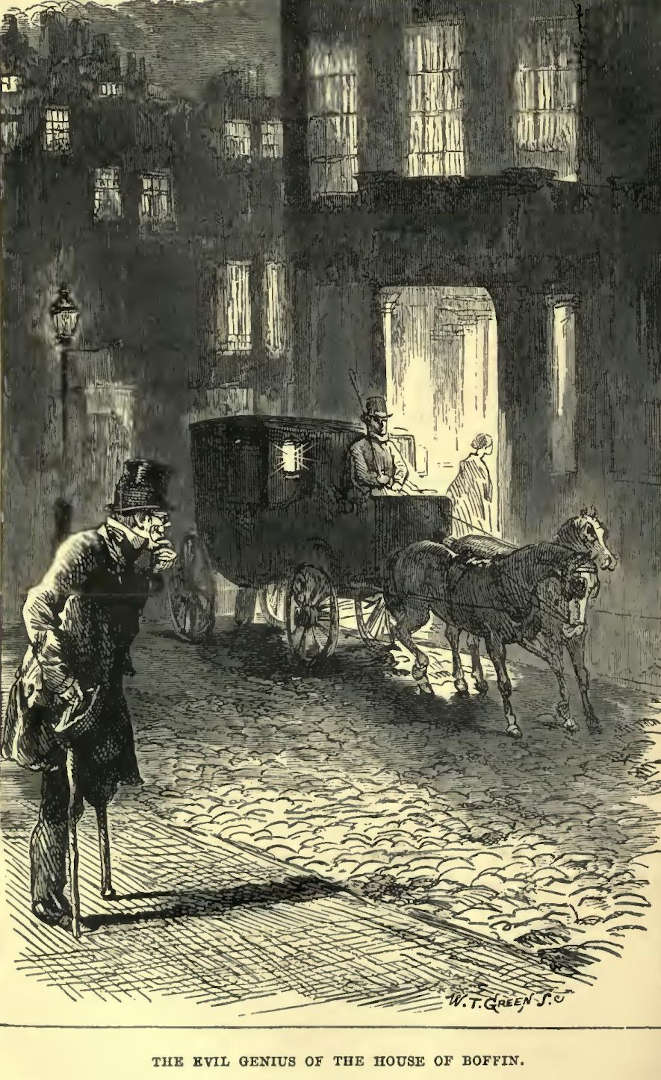
\includegraphics[scale=2.3]{03-07-01}

For, Silas Wegg felt it to be quite out of the question that he could
lay his head upon his pillow in peace, without first hovering over
Mr Boffin’s house in the superior character of its Evil Genius. Power
(unless it be the power of intellect or virtue) has ever the greatest
attraction for the lowest natures; and the mere defiance of the
unconscious house-front, with his power to strip the roof off the
inhabiting family like the roof of a house of cards, was a treat which
had a charm for Silas Wegg.

As he hovered on the opposite side of the street, exulting, the carriage
drove up.

‘There’ll shortly be an end of YOU,’ said Wegg, threatening it with the
hat-box. ‘YOUR varnish is fading.’

Mrs Boffin descended and went in.

‘Look out for a fall, my Lady Dustwoman,’ said Wegg.

Bella lightly descended, and ran in after her.

‘How brisk we are!’ said Wegg. ‘You won’t run so gaily to your old
shabby home, my girl. You’ll have to go there, though.’

A little while, and the Secretary came out.

‘I was passed over for you,’ said Wegg. ‘But you had better provide
yourself with another situation, young man.’

Mr Boffin’s shadow passed upon the blinds of three large windows as he
trotted down the room, and passed again as he went back.

‘Yoop!’ cried Wegg. ‘You’re there, are you? Where’s the bottle? You
would give your bottle for my box, Dustman!’

Having now composed his mind for slumber, he turned homeward. Such
was the greed of the fellow, that his mind had shot beyond halves,
two-thirds, three-fourths, and gone straight to spoliation of the whole.
‘Though that wouldn’t quite do,’ he considered, growing cooler as he got
away. ‘That’s what would happen to him if he didn’t buy us up. We should
get nothing by that.’

We so judge others by ourselves, that it had never come into his head
before, that he might not buy us up, and might prove honest, and prefer
to be poor. It caused him a slight tremor as it passed; but a very
slight one, for the idle thought was gone directly.

‘He’s grown too fond of money for that,’ said Wegg; ‘he’s grown too fond
of money.’ The burden fell into a strain or tune as he stumped along the
pavements. All the way home he stumped it out of the rattling streets,
PIANO with his own foot, and FORTE with his wooden leg, ‘He’s GROWN too
FOND of MONEY for THAT, he’s GROWN too FOND of MONEY.’

Even next day Silas soothed himself with this melodious strain, when he
was called out of bed at daybreak, to set open the yard-gate and admit
the train of carts and horses that came to carry off the little Mound.
And all day long, as he kept unwinking watch on the slow process which
promised to protract itself through many days and weeks, whenever
(to save himself from being choked with dust) he patrolled a little
cinderous beat he established for the purpose, without taking his eyes
from the diggers, he still stumped to the tune: He’s GROWN too FOND of
MONEY for THAT, he’s GROWN too FOND of MONEY.’



